\chapter{YAML for bnet storage}

When dealing with bnets,
it is often necessary to store
them for future reuse.
 For instance, my Mappa Mundi
software (Ref.\cite{mappa-mundi}) stores
bnets
for future reuse. I does so
continuously, 
as they are learned by the AI. The bnets are stored in a directory that I call a {\bf DAG atlas}.

In this chapter, we will discuss a language called YAML, 
and how to store bnets using YAML.



There are infinitely many ways of storing a bnet. 
The reasons why we propose using the YAML
language is that it is a popular,
standardized,
human readable, and fairly succinct language.

The configuration information of a software app, and the data exchanged between apps,  is often stored in a  YAML data structure.

\begin{figure}[h!]
\centering
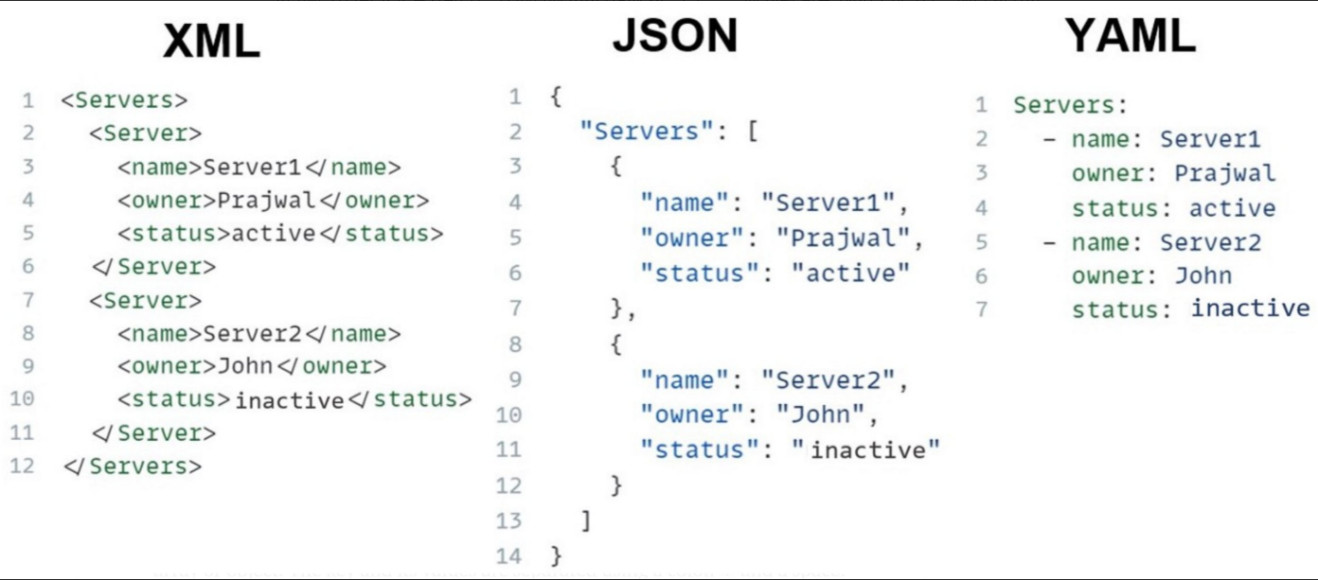
\includegraphics[width=6in]
{yaml/json-xml-yaml.jpg}
\caption{For simple data structures,
one can translate between JSON, XML and YAML.}
\label{fig-json-xml-yaml}
\end{figure}

YAML is a human-readable data serialization language.
XML and JSON are too.
As illustrated by Fig.\ref{fig-json-xml-yaml}, for simple data structures, one can translate a data structure
from one of those languages to the other 2. 
But note that
YAML is the most succinct 
language of the 3.
So in this chapter, we will speak only about YAML.

\section{Getting acquainted with YAML}
In Chapter \ref{ch-dtree},
we demonstrated that a (decision) tree
can be converted without loss of
information to a bnet with the
same structure as the tree.
This is done by using marginalizer nodes.

The purpose of this section is not to teach
YAML to the reader.
In this section, we will
assume that the reader has learned YAML already,
from one of many excellent introductions to YAML
available on the internet.


The purpose of this section is to
demonstrate that a YAML data structure can be converted to
a tree. Then using
the results of Chapter \ref{ch-dtree}, that tree can be converted to a decision tree which can be converted to a bnet.

Like Python, YAML code 
can contain 2 data structures: dictionaries
such as 

$$\boxed{\begin{array}{l}
{\tt a:1}\\
{\tt b:5}\\
{\tt c:1}
\end{array}}
\leftrightarrow
{\tt \{a:1,\quad b:5,\quad c:1\}} 
$$
and lists such as

$$
\boxed{
\begin{array}{l}
{\tt - \quad x}\\
{\tt -\quad y}\\
{\tt -\quad z}
\end{array}}
\leftrightarrow
{\tt [x,\quad y,\quad z]}
$$
In YAML, the dictionaries
have all their key-value
pairs start with the same level of indentation.
The list items also start with
the same level of indentation, but all start with a hyphen and a space.
Lists can always be replaced by dictionaries:

$${\tt [x,\quad y,\quad z] \rarrow
\{0:x, \quad 1:y,\quad 2:z\}}
$$

$$
\boxed{
\begin{array}{l}
{\tt - \quad x}\\
{\tt -\quad y}\\
{\tt -\quad z}
\end{array}}
\rarrow
\boxed{
\begin{array}{l}
{\tt 0: \quad x}\\
{\tt 1: \quad y}\\
{\tt 2:\quad z}
\end{array}}
$$

Once you replace in
a YAML data structure, all lists
by dictionaries,
then you have dictionaries 
with key-value pairs such that
some of the values in the pairs can lead to new dictionaries. Thus, we get a tree. See Figs.\ref{fig-yaml-list-nodes}
and \ref{fig-yaml-dict-nodes}
for examples of conversions
of YAML data structures to trees.


\begin{figure}[h!]
\centering
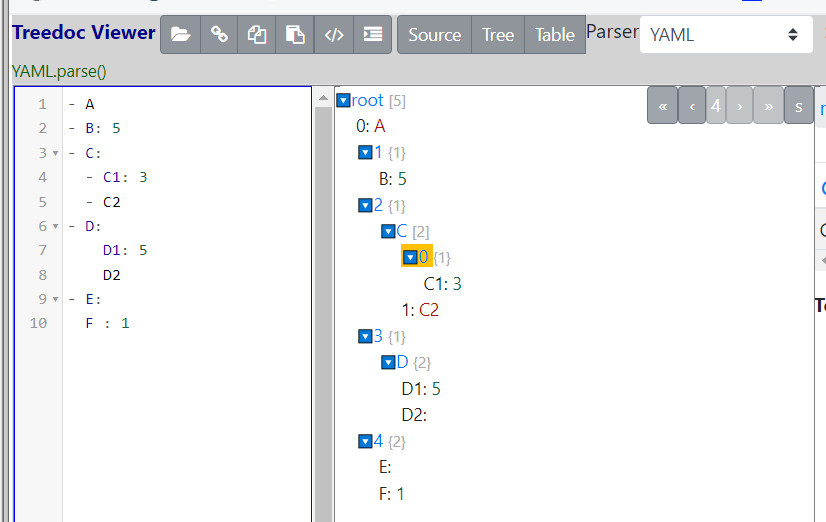
\includegraphics[width=6in]
{yaml/yaml-list-nodes.jpg}
\caption{The  nodes of a YAML list can contain various cargoes.}
\label{fig-yaml-list-nodes}
\end{figure}

\begin{figure}[h!]
\centering
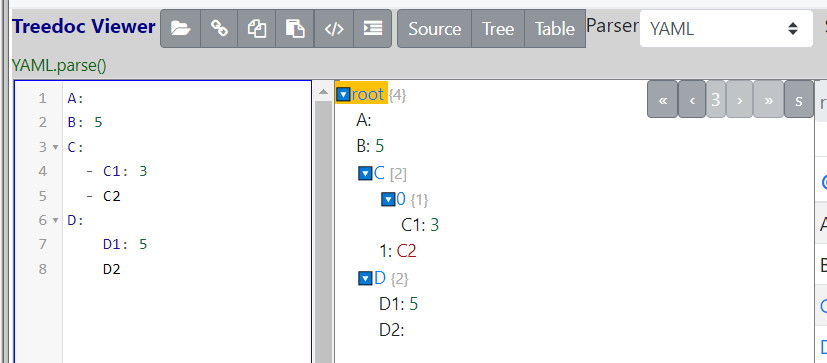
\includegraphics[width=6in]
{yaml/yaml-dict-nodes.jpg}
\caption{The nodes of a YAML dictionary can contain various cargoes. }
\label{fig-yaml-dict-nodes}
\end{figure}

\section{Storing Bnets}

As an example, below is a
possible way of
fully specifying the LDEN
 bnet\footnote{LDEN bnets are defined in Chapter \ref{ch-linear-sys}}:

$$
\xymatrix{
&\ul{A}\ar[dl]_3\ar[dr]^5
\\
\ul{B}\ar[dr]_{-6} & &\ul{C}\ar[dl]^{3} \\
&\ul{D}
}
$$
using YAML. Of course,
there are
many other ways of
doing this.

\begin{mdframed}[hidealllines=true,backgroundcolor=blue!10]
\begin{verbatim}
graph0:
  nodes:
    - id: A
      label: Node A
      values: 
        - 0 
        - 1
      parents: None
      probabilities: [0.3, 0.7]
    - id: B
      label: Node B
      values: 
        - 0 
        - 1
      parents:
        -A
      probabilities: [[0.8, 0.2], [0.6, 0.4]]
    - id: C
      label: Node C
      values:
        - 0
        - 1
      parents: 
        - A   
      probabilities: [[0.8, 0.2], [0.6, 0.4]]
    - id: D
      label: Node D
      values:
        - 0
        - 1
      parents: 
        - B
        - C
      probabilities: [[0.9, 0.1], [0.3, 0.7], [0.5, 0.5], [0.4, 0.6]]
  edge_gains:
    (A, B): 3 # arrow from A to B has gain 3
    (A, C): 5
    (B, D): -6
    (C, D): 3
\end{verbatim}
\end{mdframed}

Note that if the 
{\tt probabilities}
are given (for a bnet with 
probabilitic nodes), then
the {\tt edge\_gains} (for an LDEN) should
excluded, and vice versa.


Another thing to notice
is that the {\tt probabilities} is a tensor
representing a transition probability matrix (TPM)
$T^{[n_1], [n_2], [a]}$
with components

\beq
 T^{\nu_1, \nu_2, \alp}= P(\alp|\nu_1, \nu_2)
 \eeq
where\footnote{As usual in this book, we use the notation $[n]=[0:n]=\{0, 1, \ldots, n-1\}$}

$\nu_1\in[n_1]$= values (a.k.a. states) of parent 1,

$\nu_2\in[n_2]$= values of parent 2, 

$\alp\in[a]$= values of focus node,

where the focus node is the node
being considered, and we are assuming the focus node has 2 parents.
